\section{Camera Model}

A camera model is a projection model that approximates the function of a camera by describing a mathematical relationship between points in 3D space and its projection onto the sensor grid of the camera. In order to accurately model a camera, we must first understand the general workings of a camera.

\begin{figure}[h!]
    \centering
    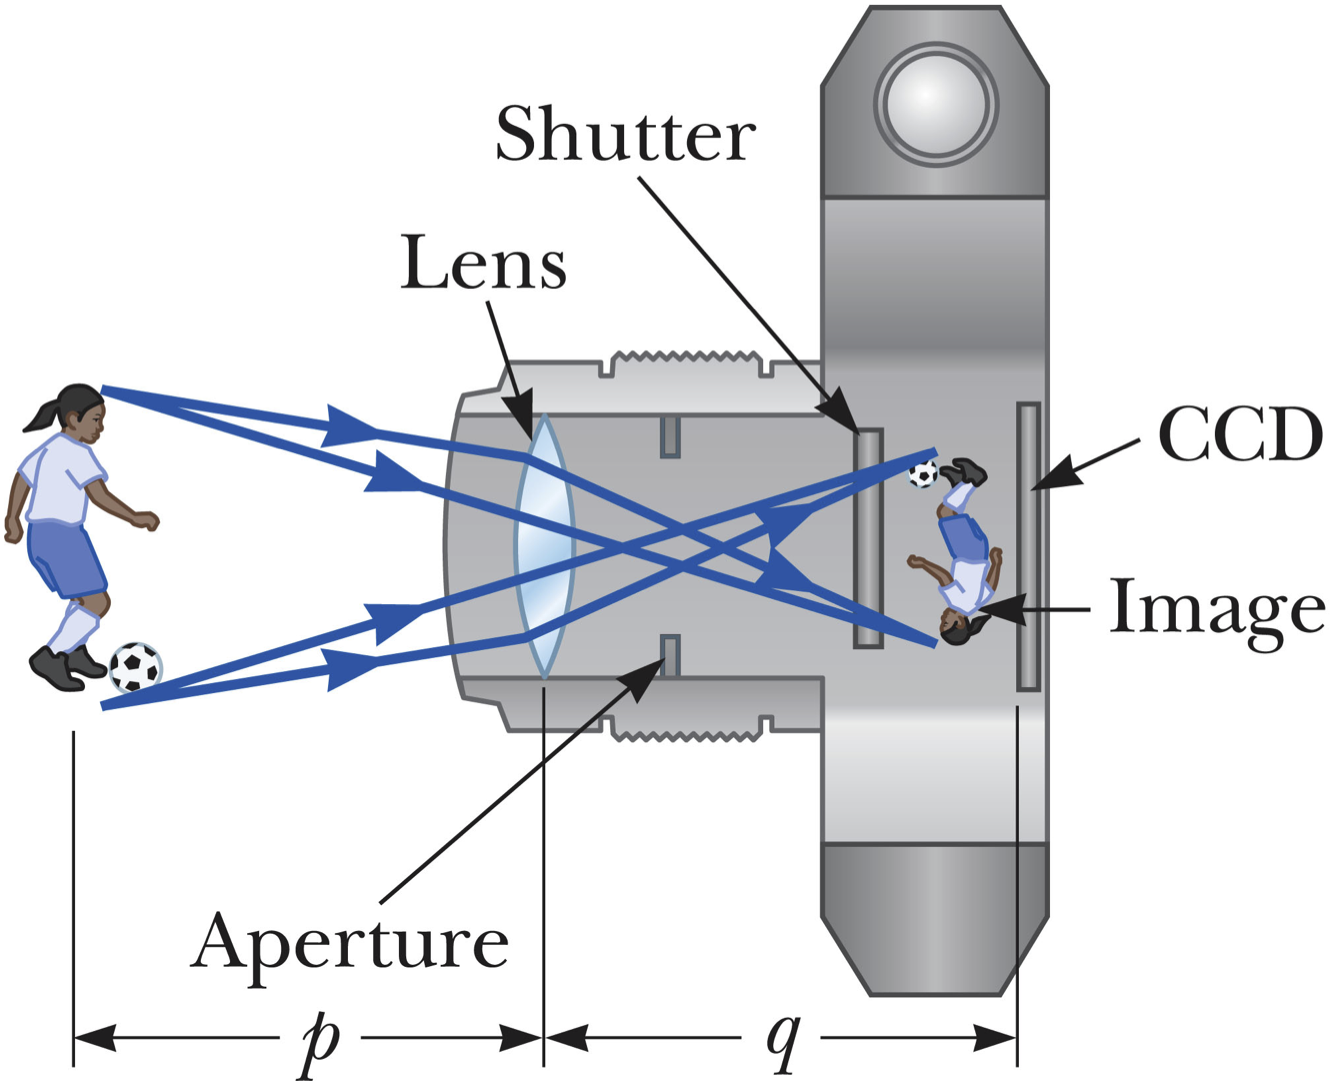
\includegraphics[width=0.5\textwidth]{images/lens_camera}
    \caption{Lens camera. Adapted from \cite{coltonPhysics1232012}} \label{fig:lens_camera}
\end{figure}


Modern lens cameras are very complex, as they often contain a series of different shaped lenses. This is an effort to compensate for other undesired effects, such as common phenomenon where the image quality in the center of the camera is better than the edges of image, due to the curvature of the lens. Additionally, they contain various intricate mechanisms, such as the ability to zoom the camera and other features to alter the image output. However, we can simplify the model of the lens camera by collapsing the mechanisms of the camera into 3 main functional components that are important to the image projection: the lens, the aperture, and the sensor grid (CCD). This simplified model is visualized in Figure \ref{fig:lens_camera}. The lens focuses incoming light rays towards the aperture, before they project inverted onto the sensor grid. However, even this simplified model of a lens camera is too complex to model, as there is no simple mathematical equation which accurately describes the behavior of a lens. As such, we can further simplify our camera model by building upon the pinhole camera model, which is one of the simplest and most commonly used camera models in camera calibration.

A pinhole camera is a simple camera without a lens. Instead, it relies on the use of a tiny hole as the aperture of the camera, and light rays pass through the hole, projecting an inverted image onto the

\begin{figure}[h!]
    \centering
    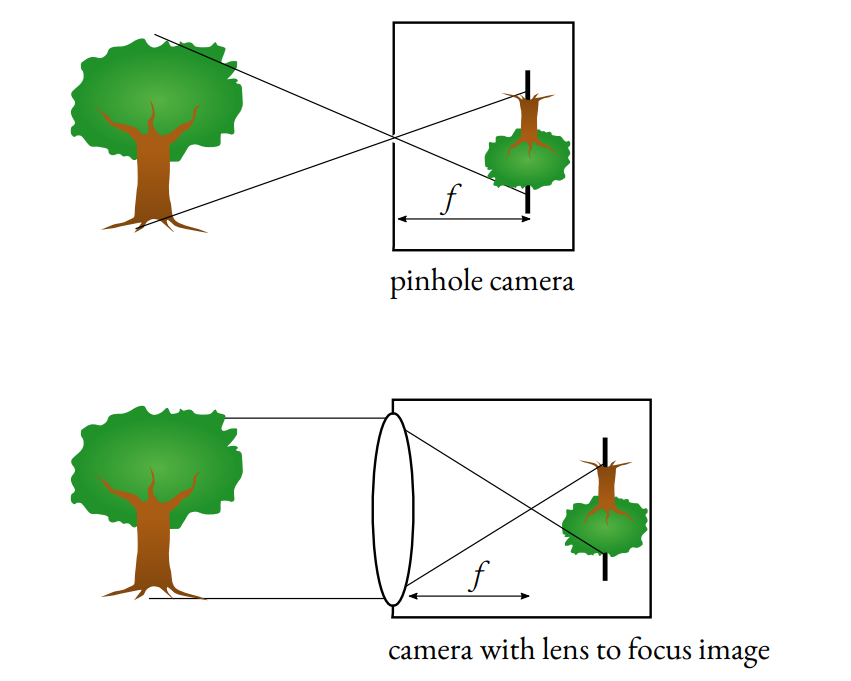
\includegraphics[width=0.7\textwidth]{images/pinhole_vs_lens}
    \caption{Difference between a pinhole camera and a lens camera. Adapted from \cite{leCameraModel2018}}
\end{figure}



There are a few assumptions which are made by the pinhole camera model:

Extremely simple model for imaging geometry
Doesn't strictly apply
Mathematically convenient acceptable approximation.
\begin{itemize}
    \item T
\end{itemize}

The pinhole camera model does not accurately describe the true workings of a camera, as some of the  effects that the model fails to account for can be compensated the errors which results from these assumptions are sufficiently small to be neglected if a high quality camera is used. Additionally,

\begin{figure}[h!]
    \centering
    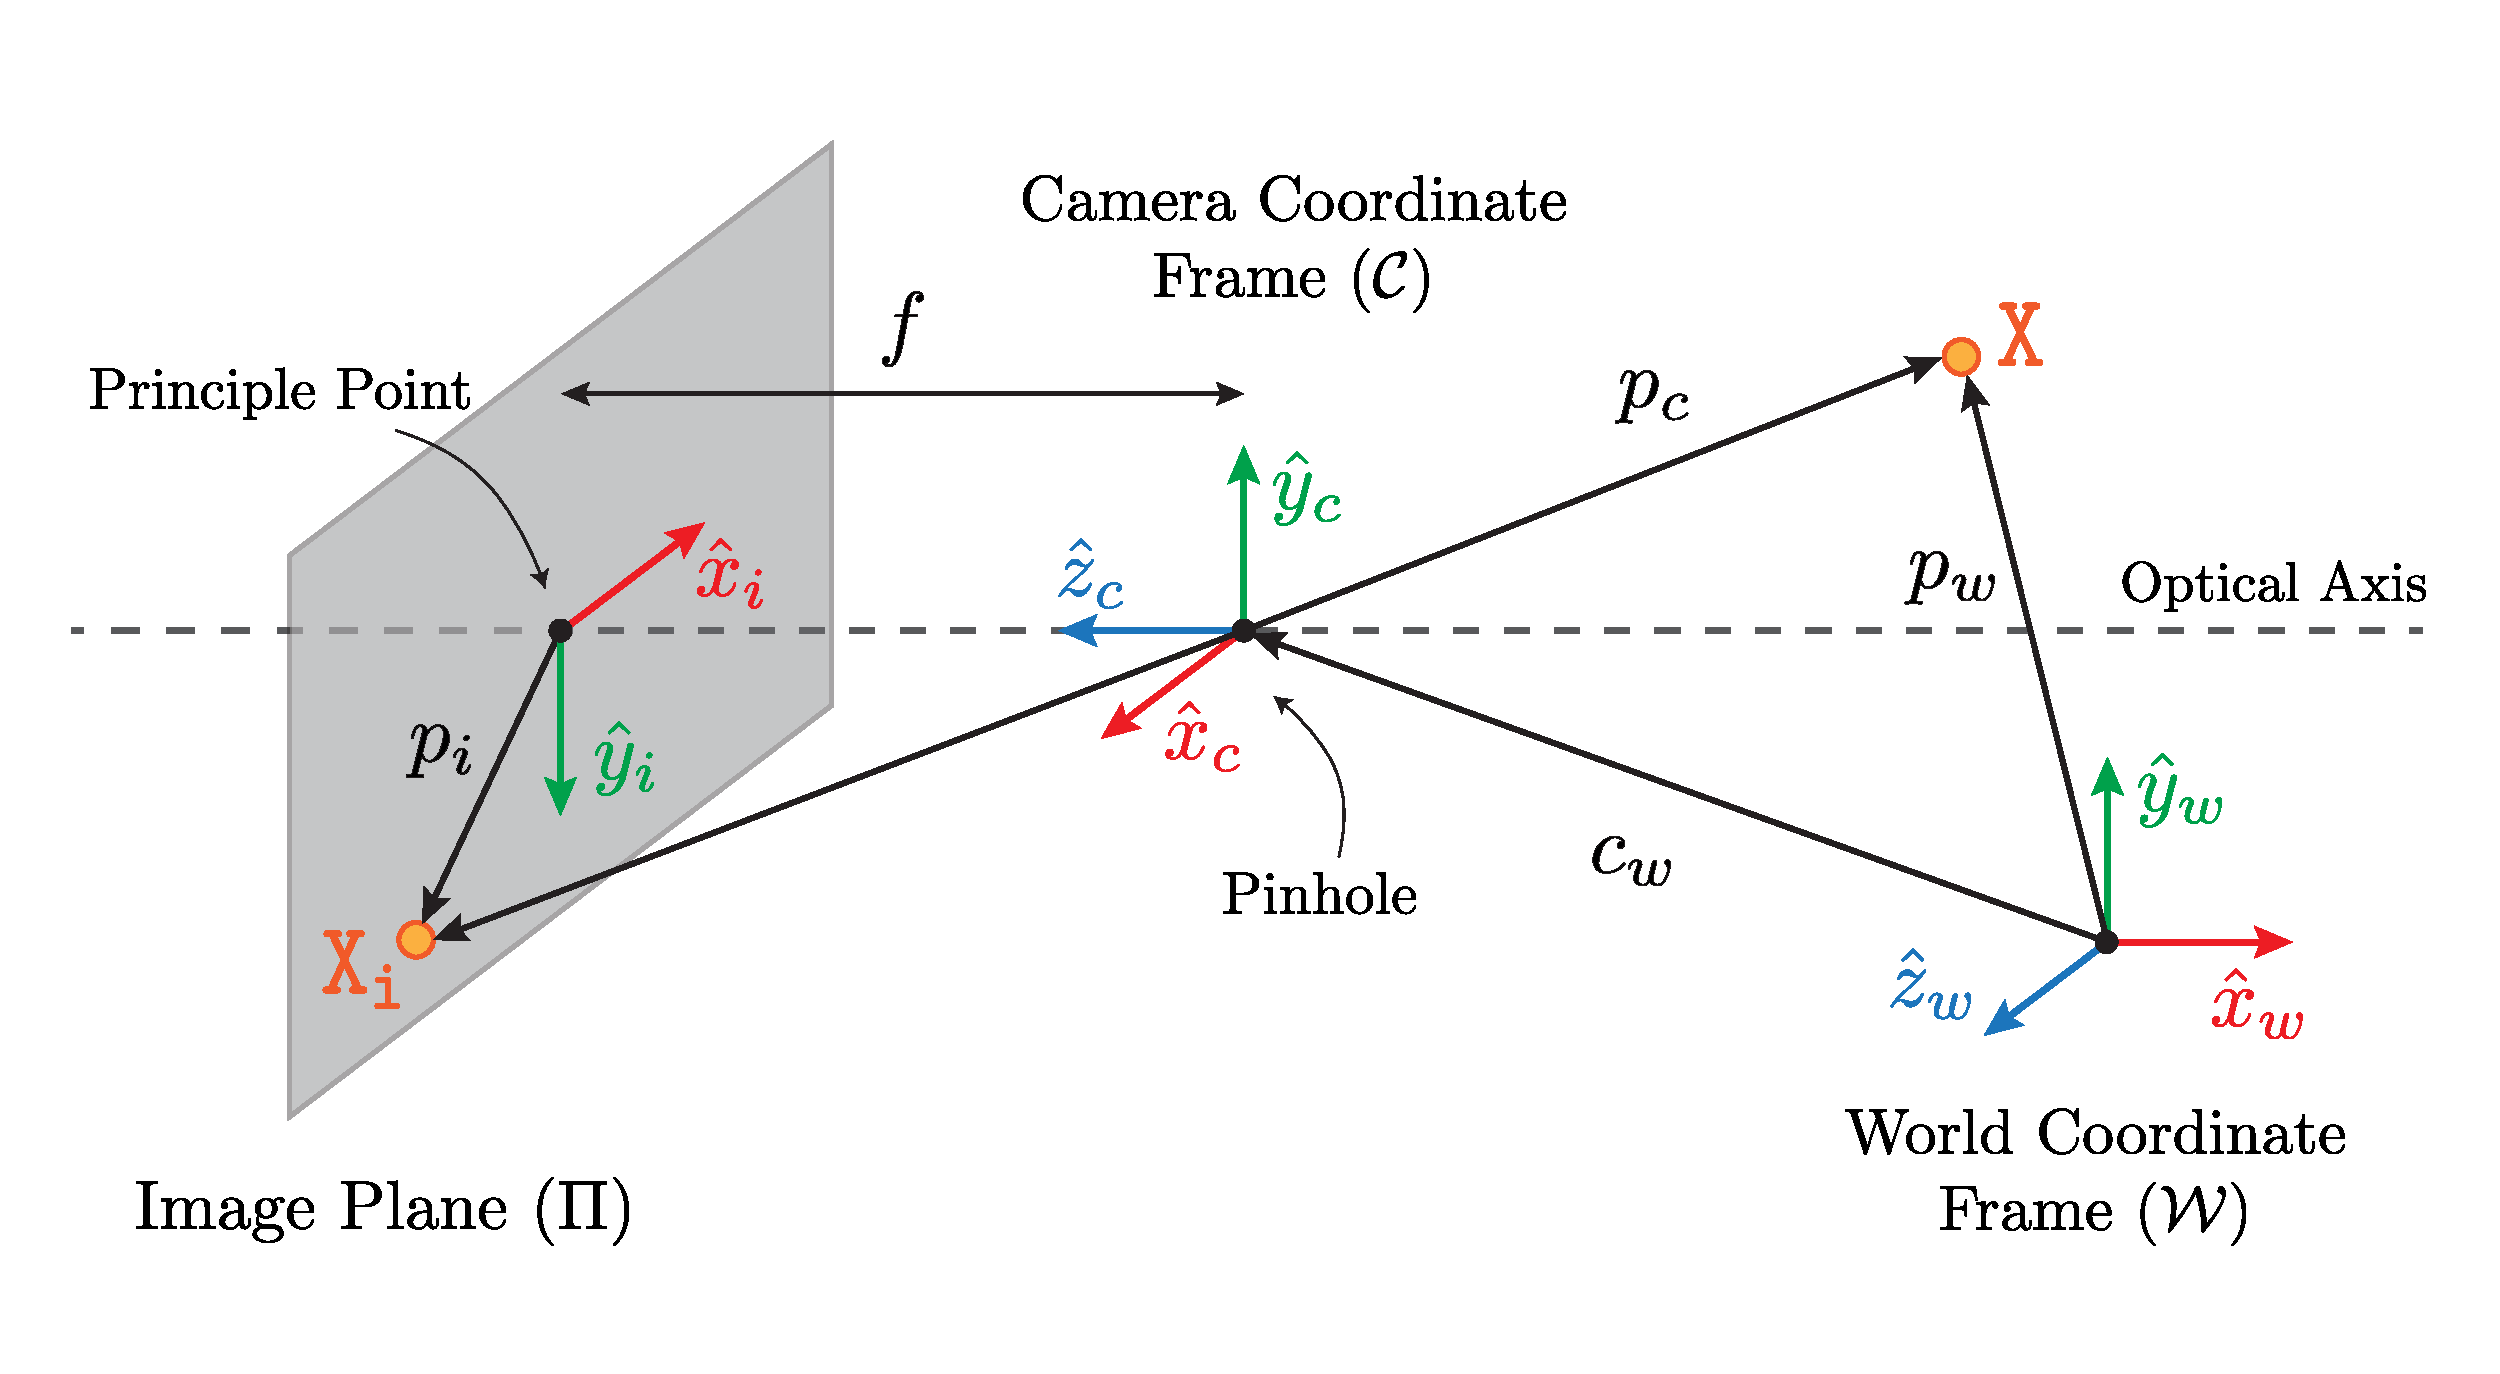
\includegraphics[width=0.9\textwidth]{figures/imaging_model}
    \caption{Pinhole camera model.}
\end{figure}

\subsection{Straetgy}

\subsection{Nomenclature}


For our camera model, we will establish 3 frames of


\begin{figure}[h!]
    \centering
    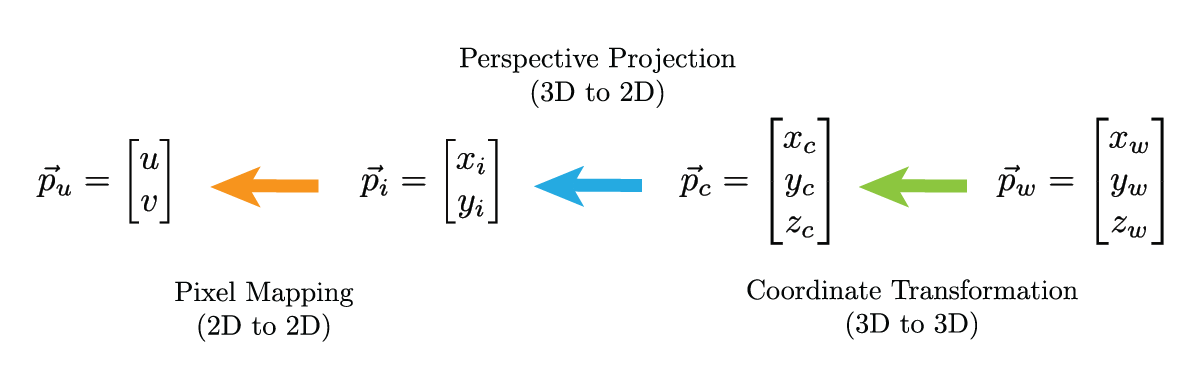
\includegraphics[width=0.9\textwidth]{figures/coord_conversions}
    \caption{Coordinate remappings.}
\end{figure}



